\section{Diseño}
\subsection[Diagrama de clases]{Diagrama de clases}
En este apartado se mostrarán los diagramas de clases de los elementos más importantes de la aplicación.\newline

En la figura \ref{fig:fragment_diagram} se muestra el diagrama de clases del Fragment (ver explicación en el glosario de la \autoref{sec:glosario}) \enquote*{TypesFragment} . Dicho diagrama de clases muestra las siguientes clases:
\begin{itemize}
	\item La clase \textbf{TypesFragment}: esta clase es la encargada de comunicar los elementos gráficos que se encuentra dentro de la lista de alojamientos y POIs, también del botón que inicia el algoritmo de búsqueda de la ruta óptima.
	\item La clase \textbf{TypesRecyclerFragment}: es la encargada de manejar la lista de alojamientos y POIs, además devuelve los elementos seleccionados en la lista al iniciar la búsqueda de la ruta. También se encarga de gestionar la interfaz gráfica de la lista.
	\item La clase \textbf{CityNodesViewHolder}: es la encargada de gestionar los elementos gráficos de los POIs o los alojamientos de forma individual.
	\item La clase \textbf{TypeViewHolder}: es la encargada de gestionar los elementos gráficos de los tipos que aparecen en la lista de alojamientos y POIs.
	\item La clase \textbf{CityNode}: clase que contiene toda la información importante sobre un alojamiento o punto de interés que se muestra en la lista.
	\item La clase \textbf{TypeOfNode}: clase que contiene la información sobre un tipo, dicho tipo engloba a POIs del mismo tipo (por ejemplo: tipo Alojamiento).
\end{itemize}
\vspace{0.06in}
En la figura  \ref{fig:main_activity_diagram}, se muestra el diagrama de clases de la actividad principal de la aplicación. Las clases que se muestran en el diagrama son las siguientes:
\begin{itemize}
	\item La clase \textbf{MapsActivity} es la clase clase principal y gestiona el mapa que se muestra y se comunica con la clase \textbf{TypesFragment} para obtener los nodos seleccionados. Esta clase contiene vectores que almacenan información sobre los marcadores que aparecen en el mapa. Dicha información se utiliza también para obtener la matriz de distancias. También contiene otros vectores para almacenar la información contenida en la solución y se utilizan para mandar la información de la solución a la actividad \textbf{ResultActivity}.
	\item La clase \textbf{DownloadFileFromURL}: se encarga de descargar y guardar la información que devuelven las peticiones a los servidores sobre alojamientos, POIs, rutas y matriz de tiempos entre POIs. Esta clase hereda de la clase AsyncTask, lo cual le permite ejecutarse en segundo plano sin que afecte al rendimiento de la interfaz de usuario.
	\item La clase \textbf{jsonProcessor} se encarga de procesar la información que se ha guardado en ficheros tras ser descargada. Esta clase utiliza la clase \textbf{JsonParser} para procesar los archivos. Además, también hereda de la clase AsyncTask por lo que se ejecuta en segundo plano.
	\item La clase \textbf{JsonParser} se encarga de procesar archivos JSON y devuelve la información contenida en los archivos en estructuras que la aplicación puede manipular.
	\item La clase \textbf{SendNodes} se encarga de obtener la matrix de distancias entre los POIs selecionados. Para ello utiliza las clases \textbf{DownloadFileFromURL} y\textbf{ jsonProcessor}, también se ejecuta en segundo plano debido a que hereda de la clase AsyncTask.
	\item La clase\textbf{ FindSolution} se encarga de ejecutar en segundo plano el algoritmo de búsqueda de rutas y de mandar la solución a la siguiente actividad. Para ello hace uso de la clase \textbf{PathFinder} y la clase \textbf{Solution}.
	\item La clase \textbf{PathFinder} es la clase que contiene el algoritmo de búsqueda de rutas. Dicha clase obtiene la solución al problema mediante el algoritmo Greedy detallado en Alg.\ref{alg:greedy_alg} y devuelve un objeto de la clase \textbf{Solution}.
	\item La clase \textbf{Solution} es la que clase que contiene una solución al problema. Esta clase cuenta con un vector que almacena los identificadores de los puntos de la solución, así como dos vectores que almacenan las horas de entrada y de salida de cada uno de los puntos de la solución.
\end{itemize}
\vspace{0.06in}
En la figura \ref{fig:models_diagram}, se muestra el diagrama de clases del paquete models; dicho paquete está formador por clases que se utilizan para modelar diferentes estructuras dentro del proyecto. Las clases que aparecen en el diagrama son las siguientes:
\begin{itemize}
	\item La clase \textbf{Solution}: clase que contiene una solución al problema. Contiene vectores para almacenar identificadores y horarios de entrada y salida de los lugares por los que pasa la solución.
	\item La clase \textbf{ModelNode}: clase genérica que se utiliza para poder mostrar elementos tanto de la clase \textbf{CityNode} como de la clase \textbf{TypeOfNode}; ambas clases están explicadas en la descripción del primer diagrama de clases.
	\item La clase \textbf{SolutionNode}: clase que contiene el nombre, el horario de entrada y salida de un nodo de la solución. Esta clase se utiliza para encapsular los nodos de la solución y acceder a los datos a la hora de mostrar la lista de la solución.
\end{itemize}
\vspace{0.06in}
En la figura \ref{fig:result_activity_diagram} muestra el diagrama de clases de la Activity (ver explicación en el glosario de la \autoref{sec:glosario}) ResultActivity, dicha Activity se muestra cuando se obtiene una solución. Las clases que se muestran en el diagrama son las siguientes:
\begin{itemize}
	\item La clase \textbf{ResultActivity}: clase que se ocupa de leer los datos mandados por la actividad principal y procesarlos para comunicarselos a la clase \textbf{SolutionFragment}.
	\item La clase \textbf{SimpleFragmentPagerAdapter}: clase que se ocupa de ver el número de soluciones que se han encontrado y crear un objeto de la clase \textbf{SolutionFragment} para mostrar cada una de ellas.
	\item La clase \textbf{SolutionFragment}: clase que se ocupa de mostrar en un mapa los marcadores de la solución y la lista con la información específica de cada uno de los marcadores. Además se ocupa de calcular el camino entre los distintos marcadores de la solución.
\end{itemize}
\vspace{0.06in}
Por último, en la figura \ref{fig:solution_recycler_diagram} se muestra el diagrama de clases de la clase \textbf{SolutionFragment}. A continuación se describen cada una de las clases que se muestran en el diagrama:
\begin{itemize}
	\item La clase \textbf{SolutionFragment} se ha definido en la figura \ref{fig:result_activity_diagram} anterior. Es la encargada de gestionar todas las vistas que muestran la solución.
	\item La clase \textbf{FindRoutes}: clase que se encarga de mandar una petición a un servidor para obtener la ruta óptima entre los nodos de la solución y procesarla, después manda la información procesada a la clase \textbf{SolutionFragment} para que dibuje la ruta.
	\item La clase \textbf{SolutionRecyclerAdater} se encarga de manejar la lista con los nodos de la solución y de mostrarlos en una lista.
	\item La clase \textbf{SolutionNode}: clase que contiene la información sobre un nodo de la solución.
	\item La clase \textbf{SolutionNodeViewHolder}: clase que utiliza la información de un objeto de la clase \textbf{SolutionNode}  y la muestra dentro de la lista que gestiona la clase \textbf{SolutionRecyclerAdapter}.
\end{itemize}
\newpage
\begin{figure}[H]
	\centering
	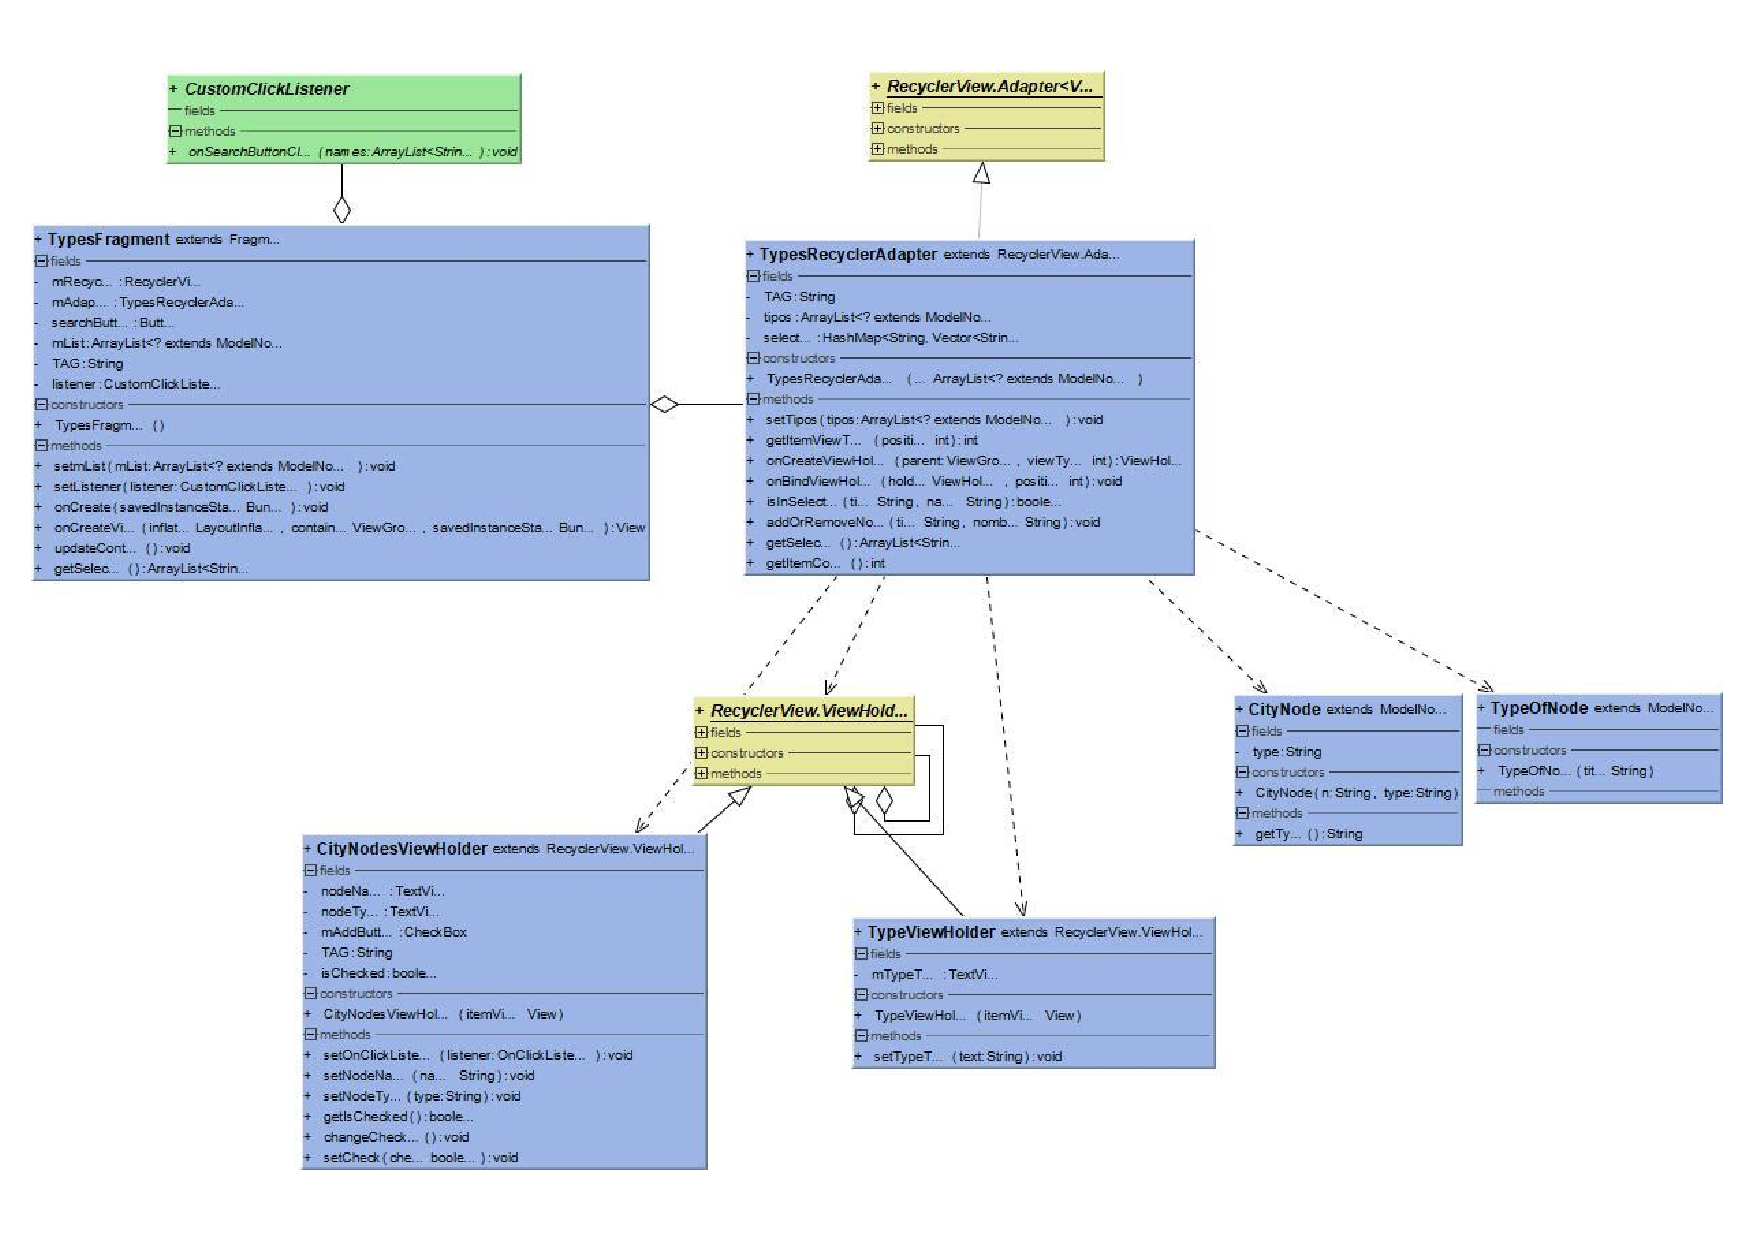
\includegraphics[scale=.8,angle=90]{imagenes/fragment_class_diagram.pdf}
	\caption{Diagrama de clases del \textbf{TypesFrament}.}
	\label{fig:fragment_diagram}
\end{figure}
\begin{figure}[H]
	\centering
	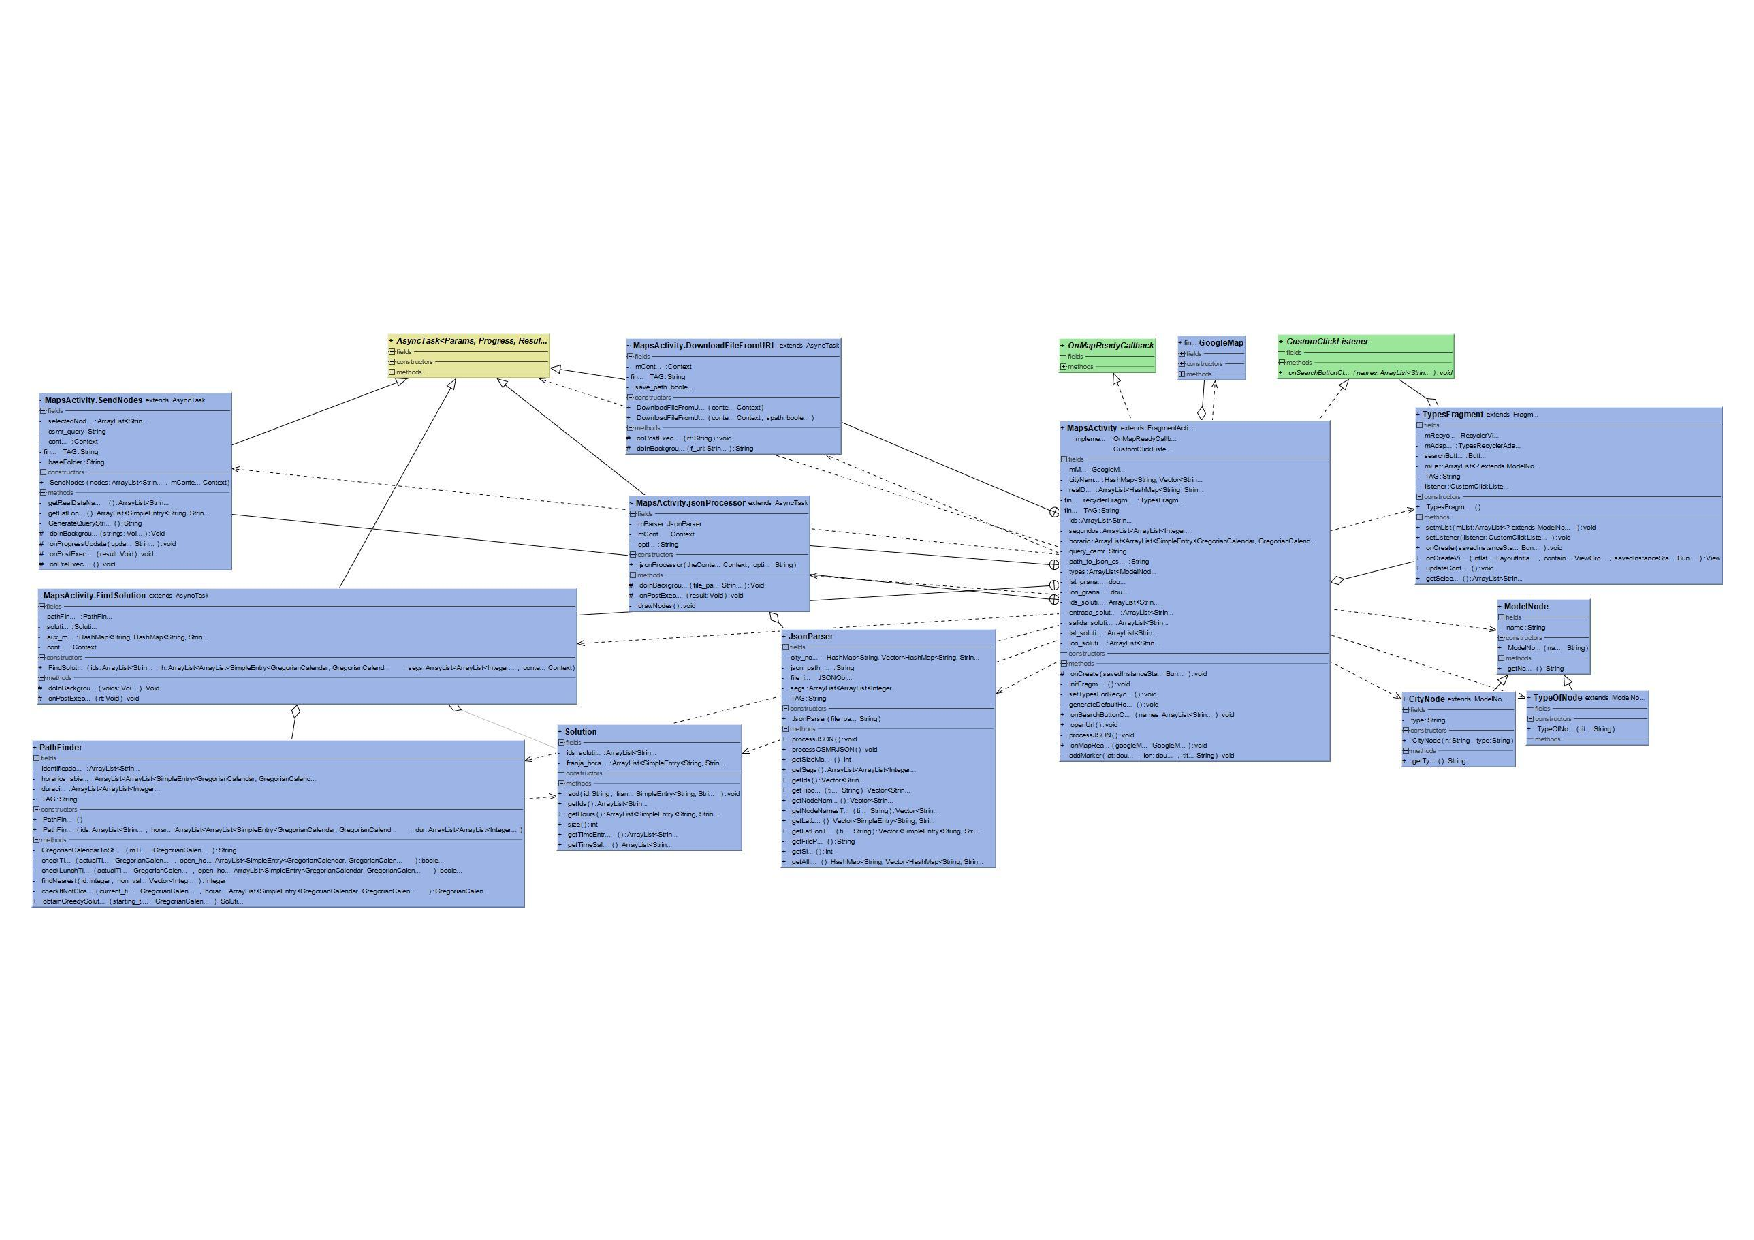
\includegraphics[scale=.8,angle=90]{imagenes/main_activity_class_diagram.pdf}
	\caption{Diagrama de clases de la actividad principal \ref{fig:anexo_diagrama_main_activity}. }
	\label{fig:main_activity_diagram}
\end{figure}
\begin{figure}[H]
	\centering
	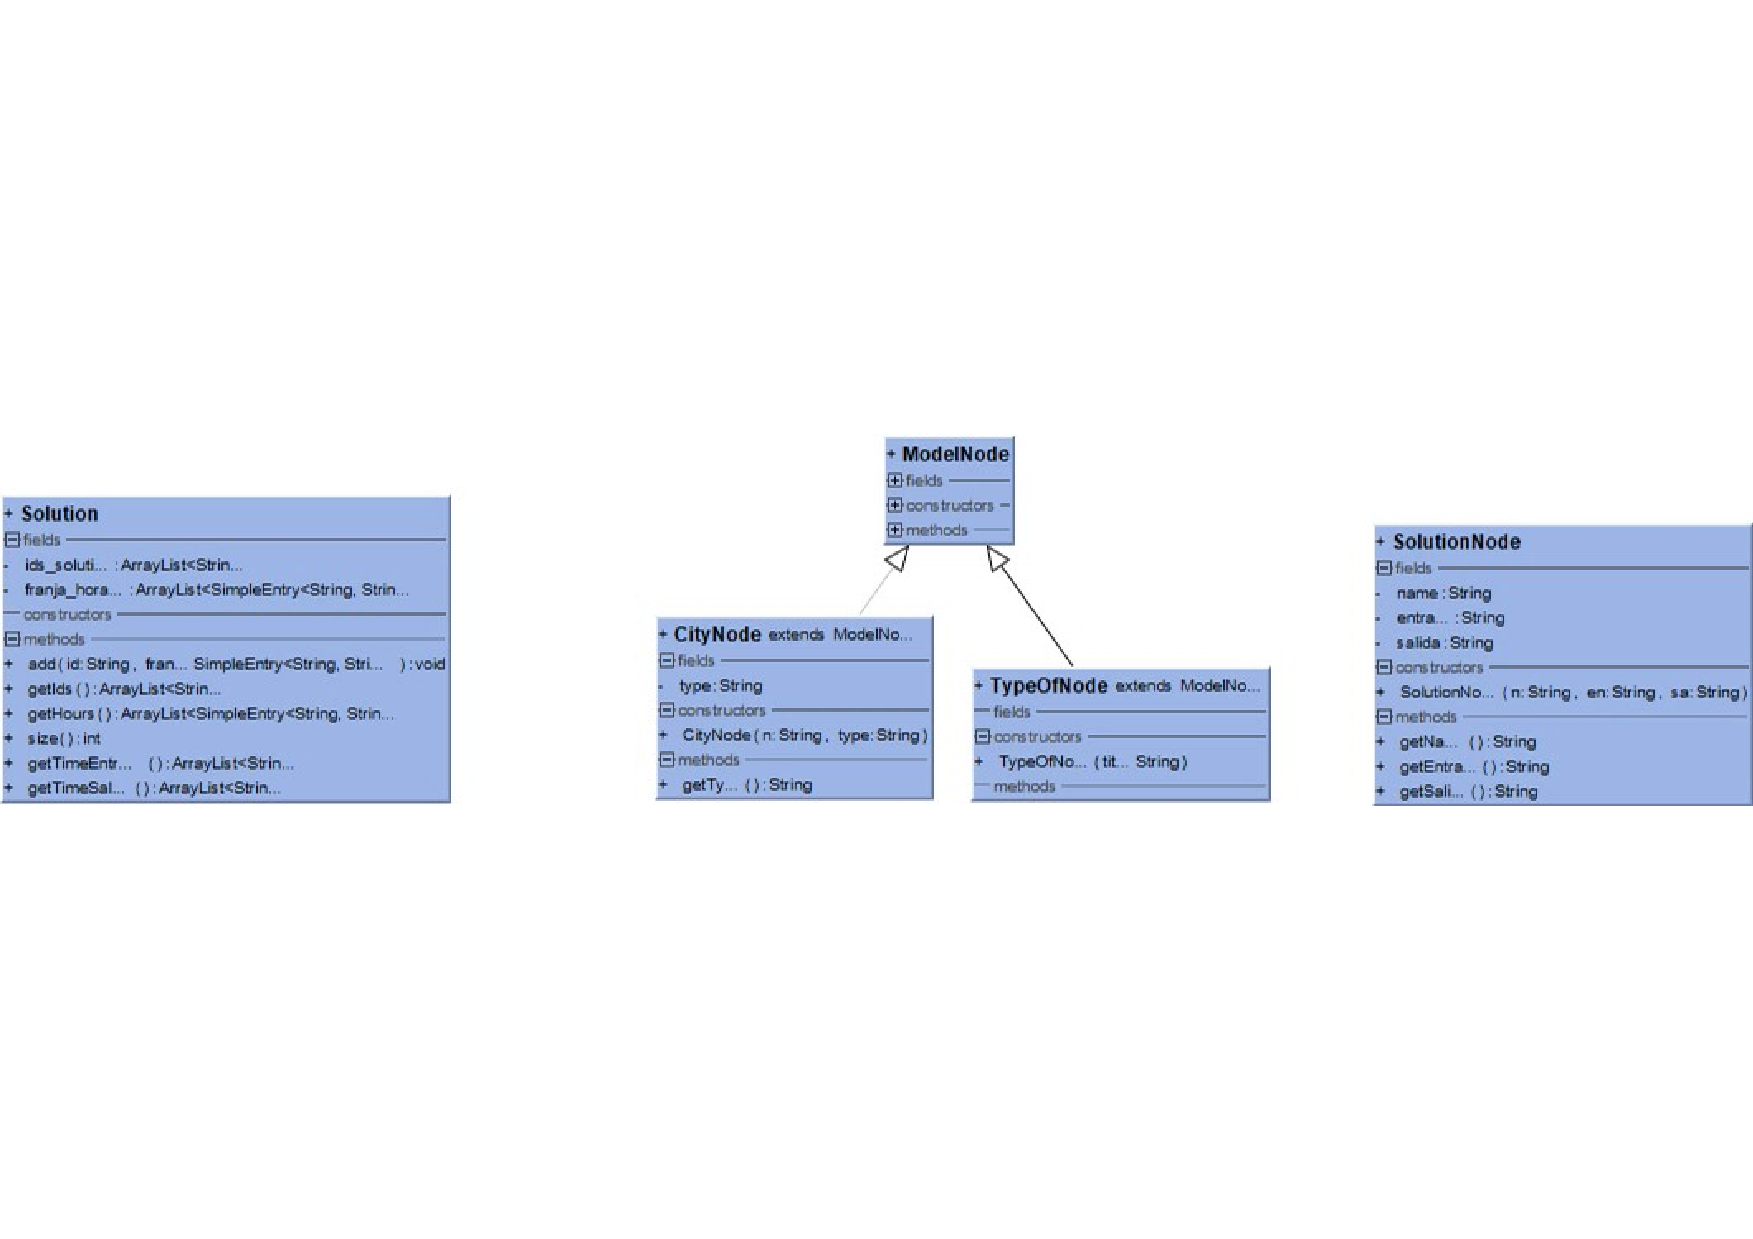
\includegraphics[scale=0.8,angle=90]{imagenes/models_package.pdf}
	\caption{Diagrama de clases del paquete \textbf{models}.}
	\label{fig:models_diagram}
\end{figure}

\begin{figure}[H]
	\centering
	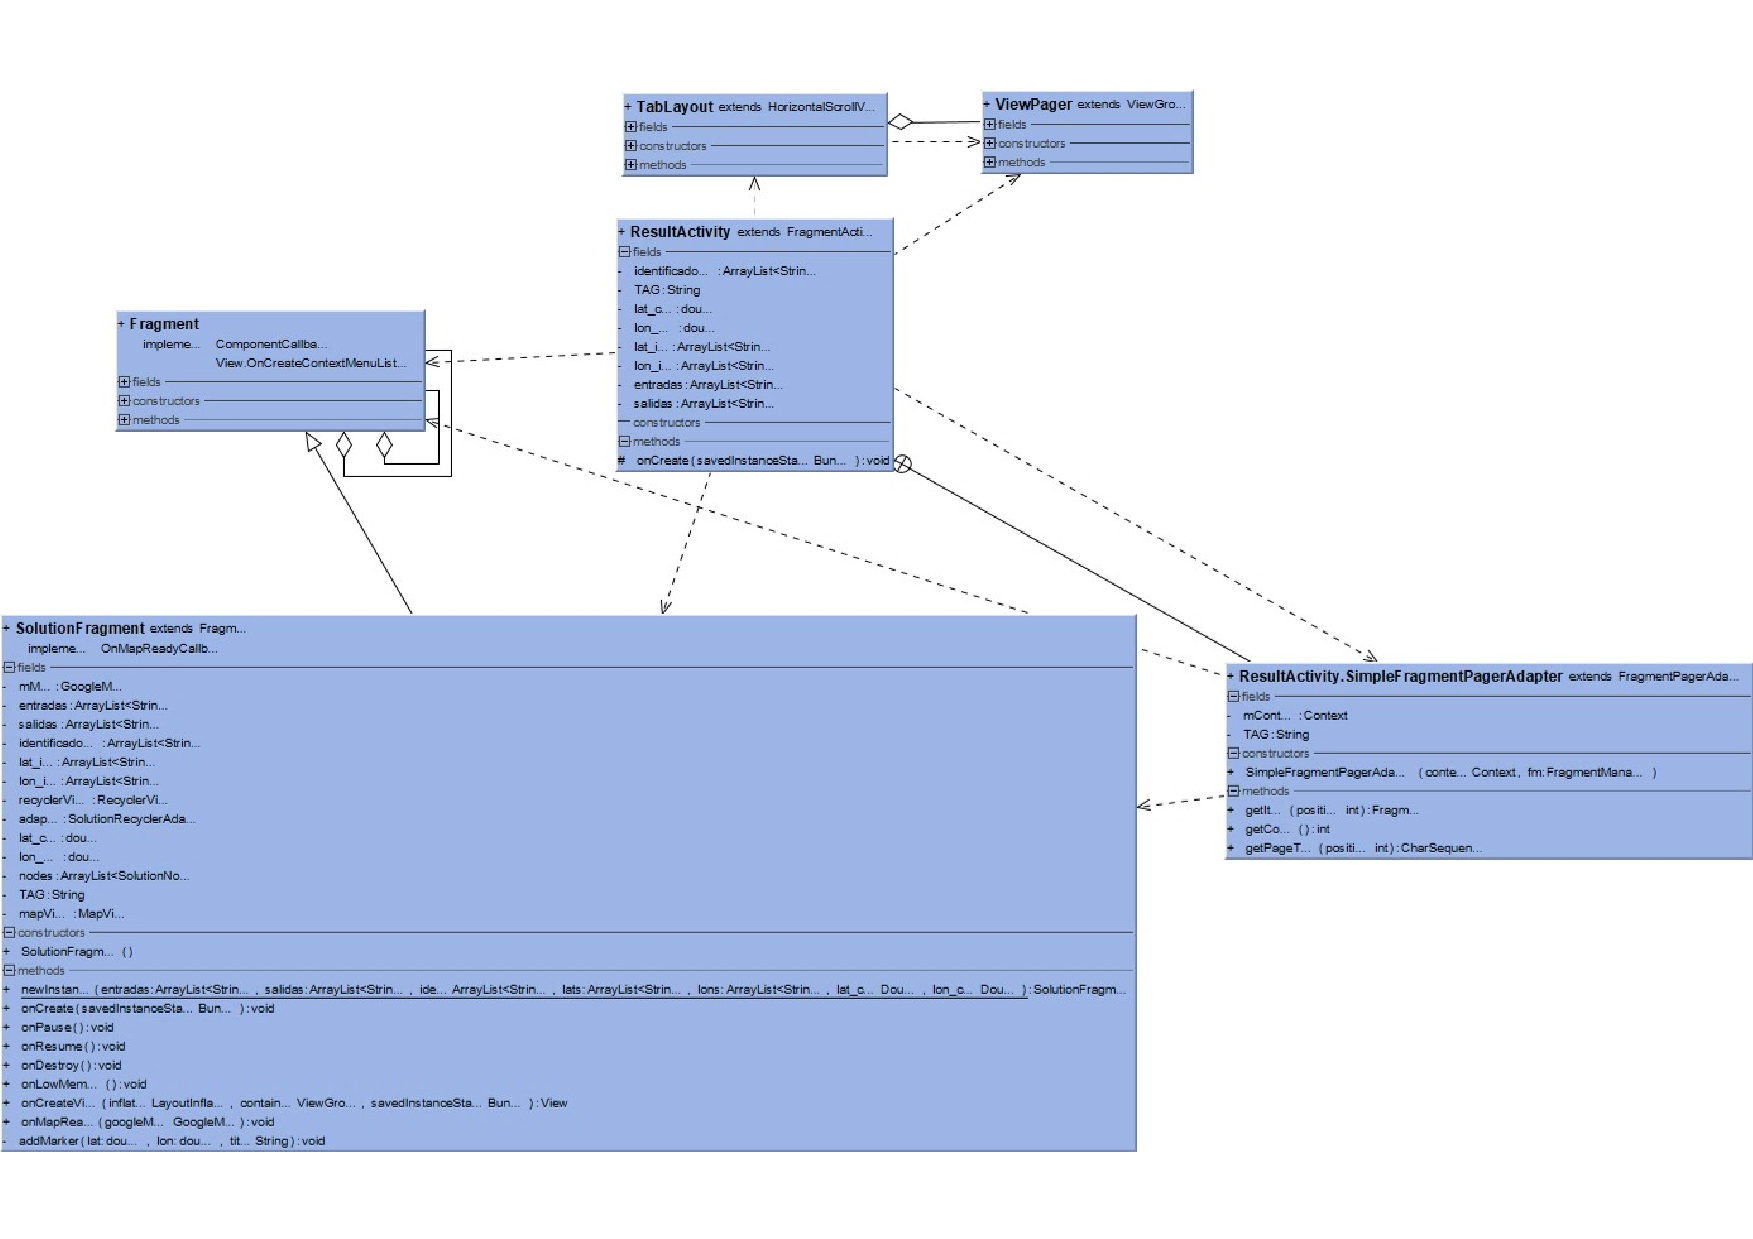
\includegraphics[scale=0.8,angle=90]{imagenes/result_activity.pdf}
	\caption{Diagrama de clases del activity \textbf{ResultActivity}.}
	\label{fig:result_activity_diagram}
\end{figure}
\begin{figure}[H]
	\centering
	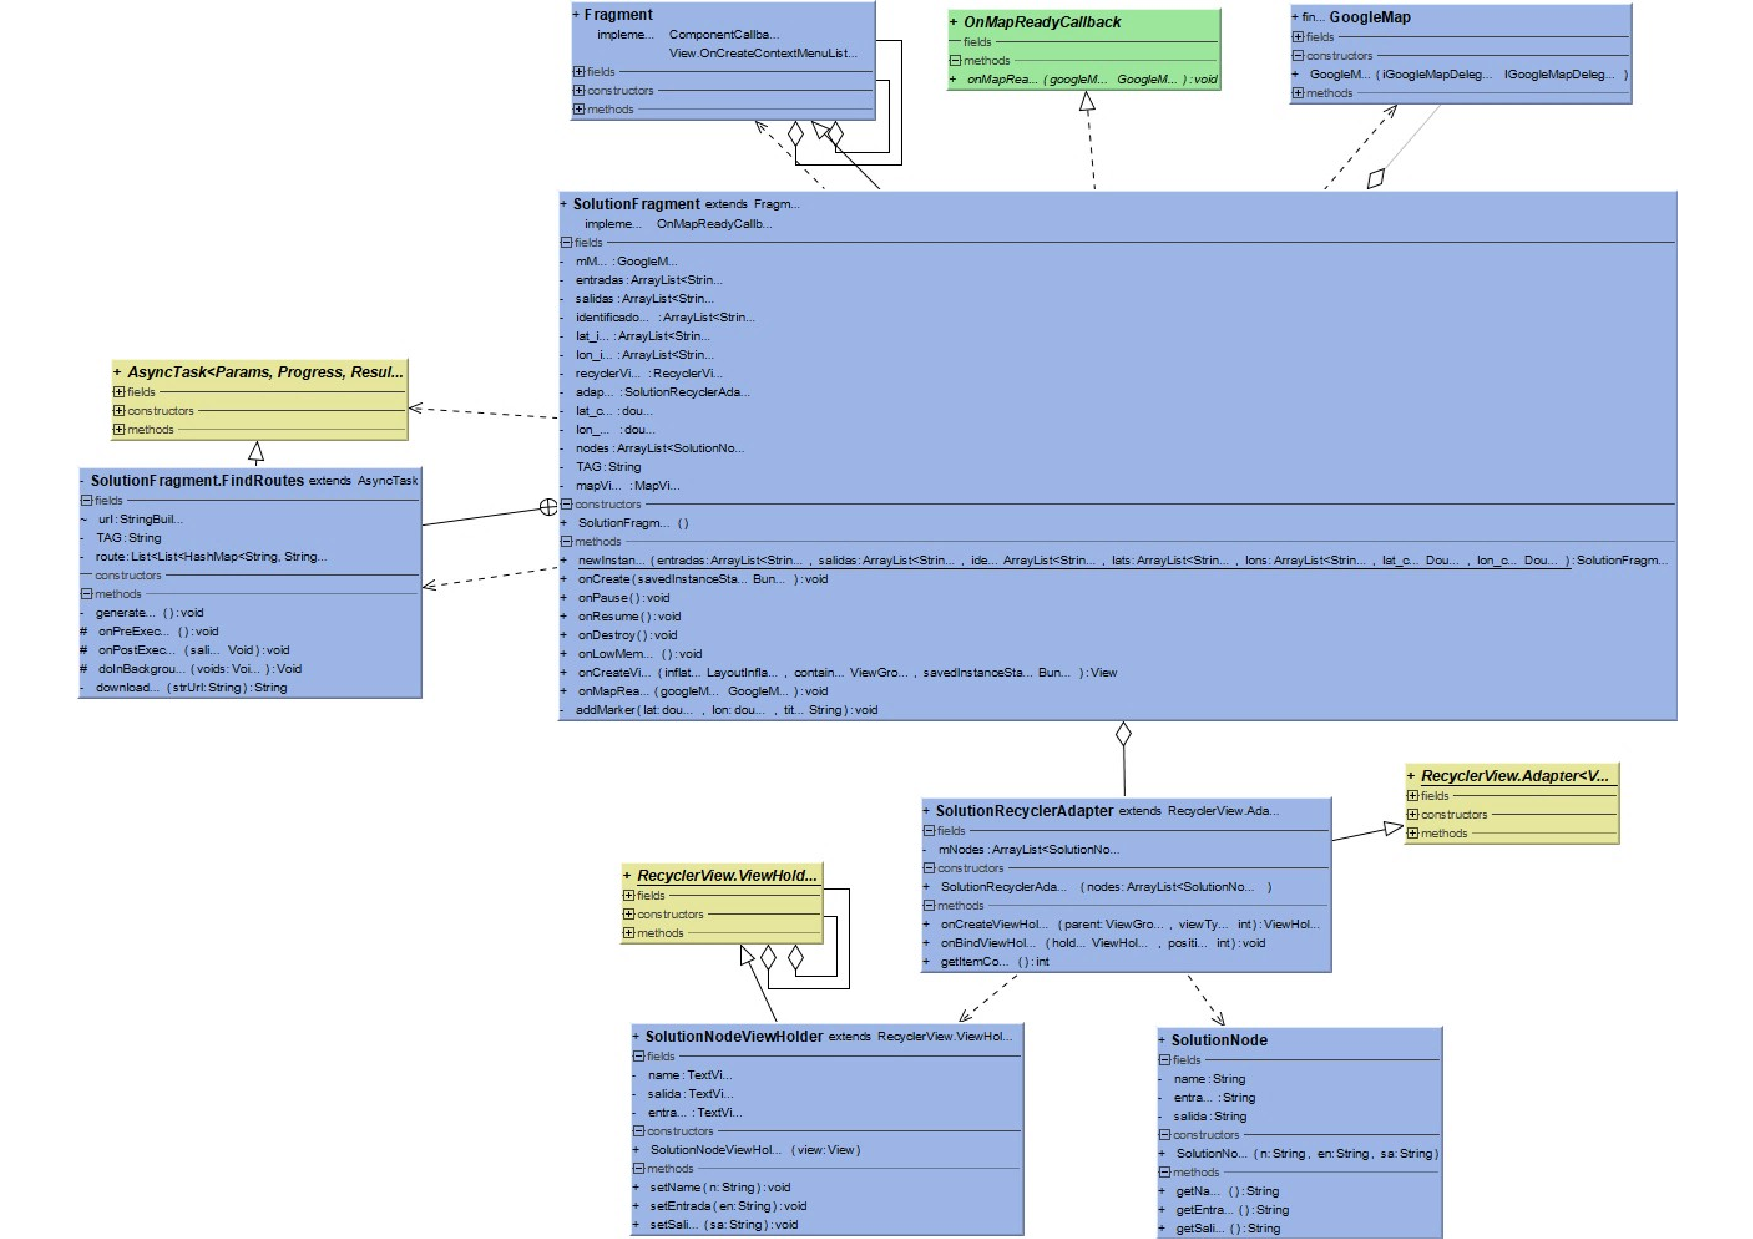
\includegraphics[scale=0.8,angle=90]{imagenes/result_fragment.pdf}
	\caption{Diagrama de clases de la clase \textbf{SolutionFragment}.}
	\label{fig:solution_recycler_diagram}
\end{figure}


\subsection[Interfaz de Usuario]{Interfaz de Usuario}

A continuación se mostrarán todos los elementos que conforman la interfaz de usuario de la aplicación.\newline

Lo primero que se muestra es la actividad principal que cuenta con un mapa, ver figura \ref{fig:main_activity_diagram}, por el que se puede navegar y una lista de alojamientos y POIs, entre los cuales el usuario puede elegir un alojamiento y el número de POIs que desee; como se muestra en la figura \ref{fig:main_activity_list}.\newline

Para poder ver la lista, se debe deslizar la pestaña \enquote*{Sitios interesantes} hacia arriba, así tendremos acceso a la lista completa, para explorar todos los alojamientos y POIs, debemos hacer scroll hacia arriba sobre la lista. Dicha lista muestra primero los alojamientos y tras estos los POIs, que se organizan en \enquote*{Museos}, \enquote*{Miradores} y \enquote*{Monumentos}.\newline

Dentro la lista, cada uno de los elementos contiene un caja en la que se puede pulsar para seleccionar o deseleccionar dicho elemento. En cada elemento de la lista, se encuentra también una caja, dicha caja permite seleccionar o deseleccionar todos los POIs de ese tipo.\newline

Tras elegir el alojamiento y los POIs que el usuario desee, se ejecuta el algoritmo. Cuando este termina se abre una nueva actividad en la cual se muestran diferentes rutas al problema. Por defecto se muestra la primera ruta, para mostrar otras rutas, se debe pulsar sobre los tabs llamados \enquote*{Solución X} para mostar otras soluciones.\newline

En la figura \ref{fig:result_activity} se muestran con marcadores los POIs seleccionados. Además, en la parte inferior de la pantalla se muestra una lista oculta que contiene la información detallada de la ruta; para poder ver dicha información se debe deslizar hacia arriba en \enquote*{Descripción ruta final} o pulsar. Dentro de la lista, se muestra en orden de visita los POIs que contiene la ruta, el primer elemento que se muestra es el alojamiento seleccionado; además, cada uno de los POIs muestra la hora aproximada de entrada y de salida de dicho POI.

\newpage
\begin{figure}[H]
	\centering
	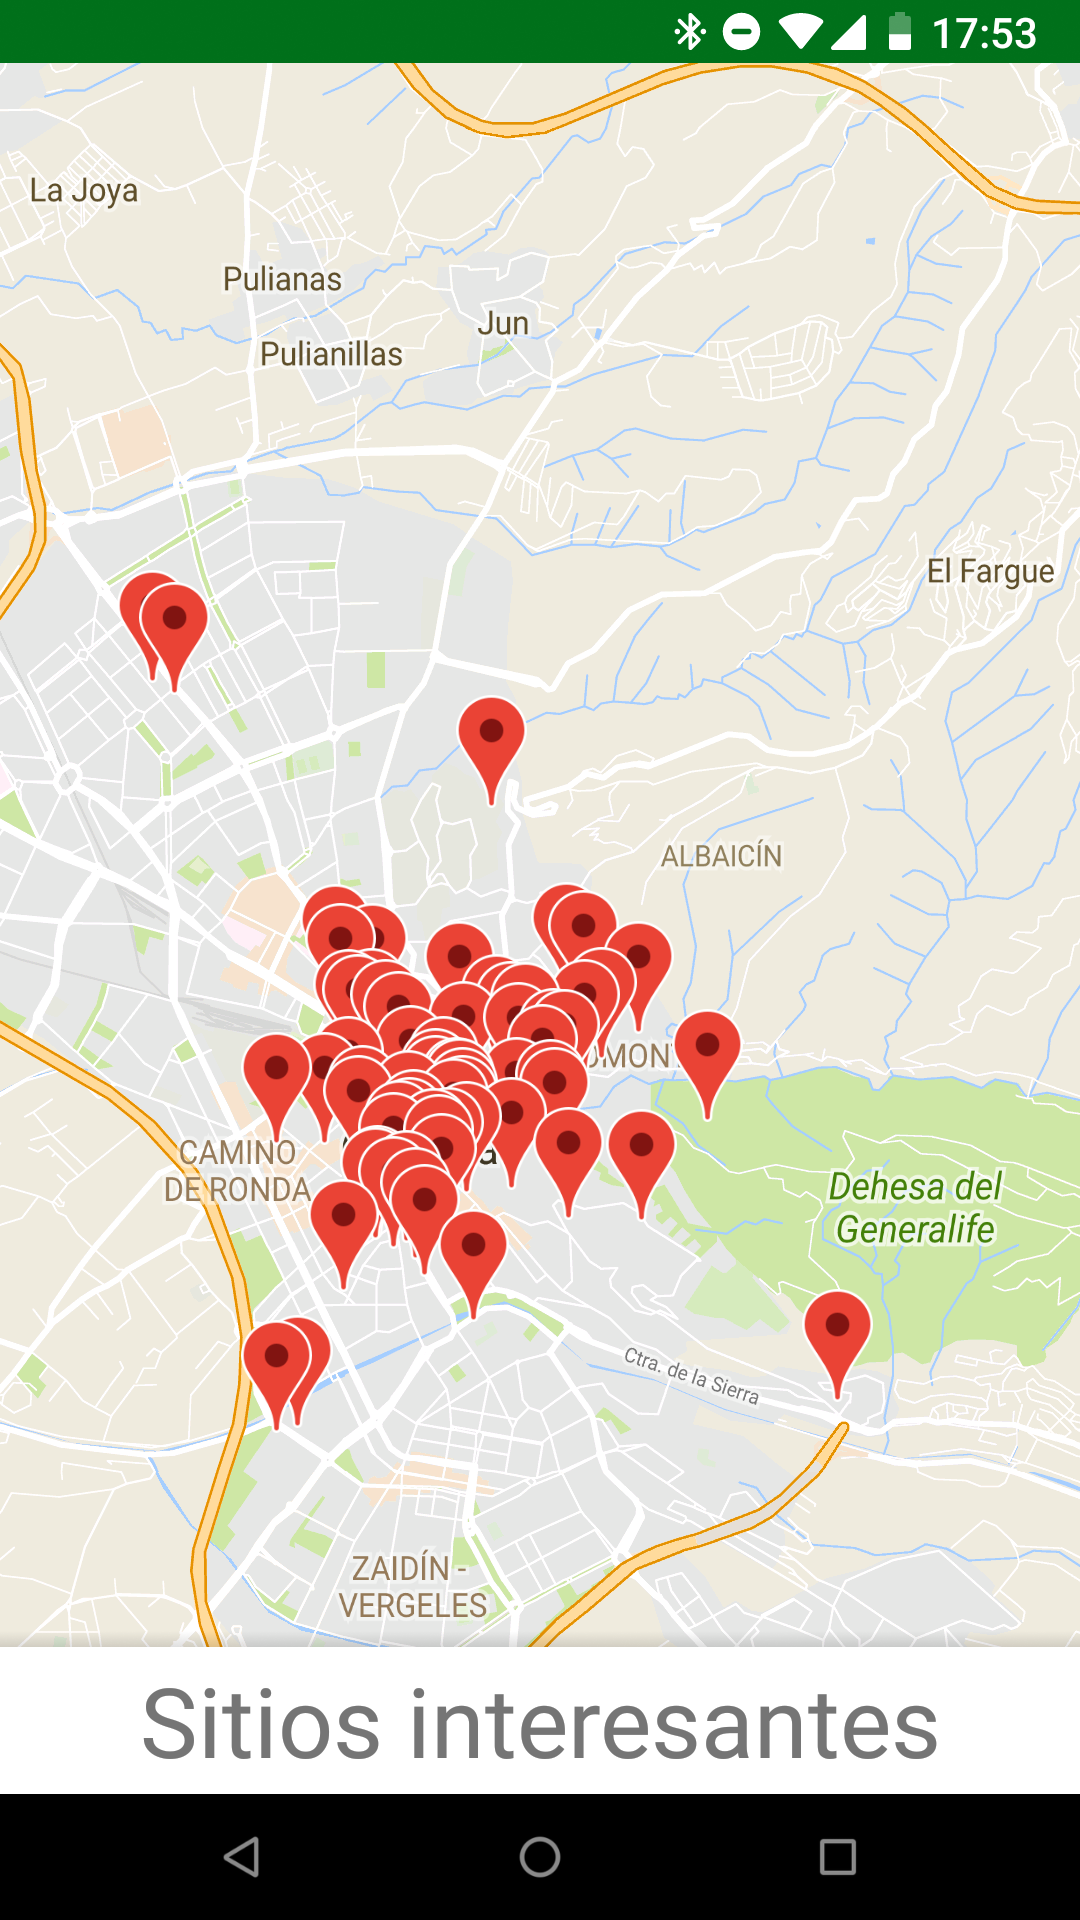
\includegraphics[width=50mm]{imagenes/main_activity_map}
	\caption{Mapa mostrando la localización de los POIs y alojamientos.}
	\label{fig:main_activity_map}
\end{figure}
\vspace{0.06in}
\begin{figure}[H]
	\centering
	\subfigure{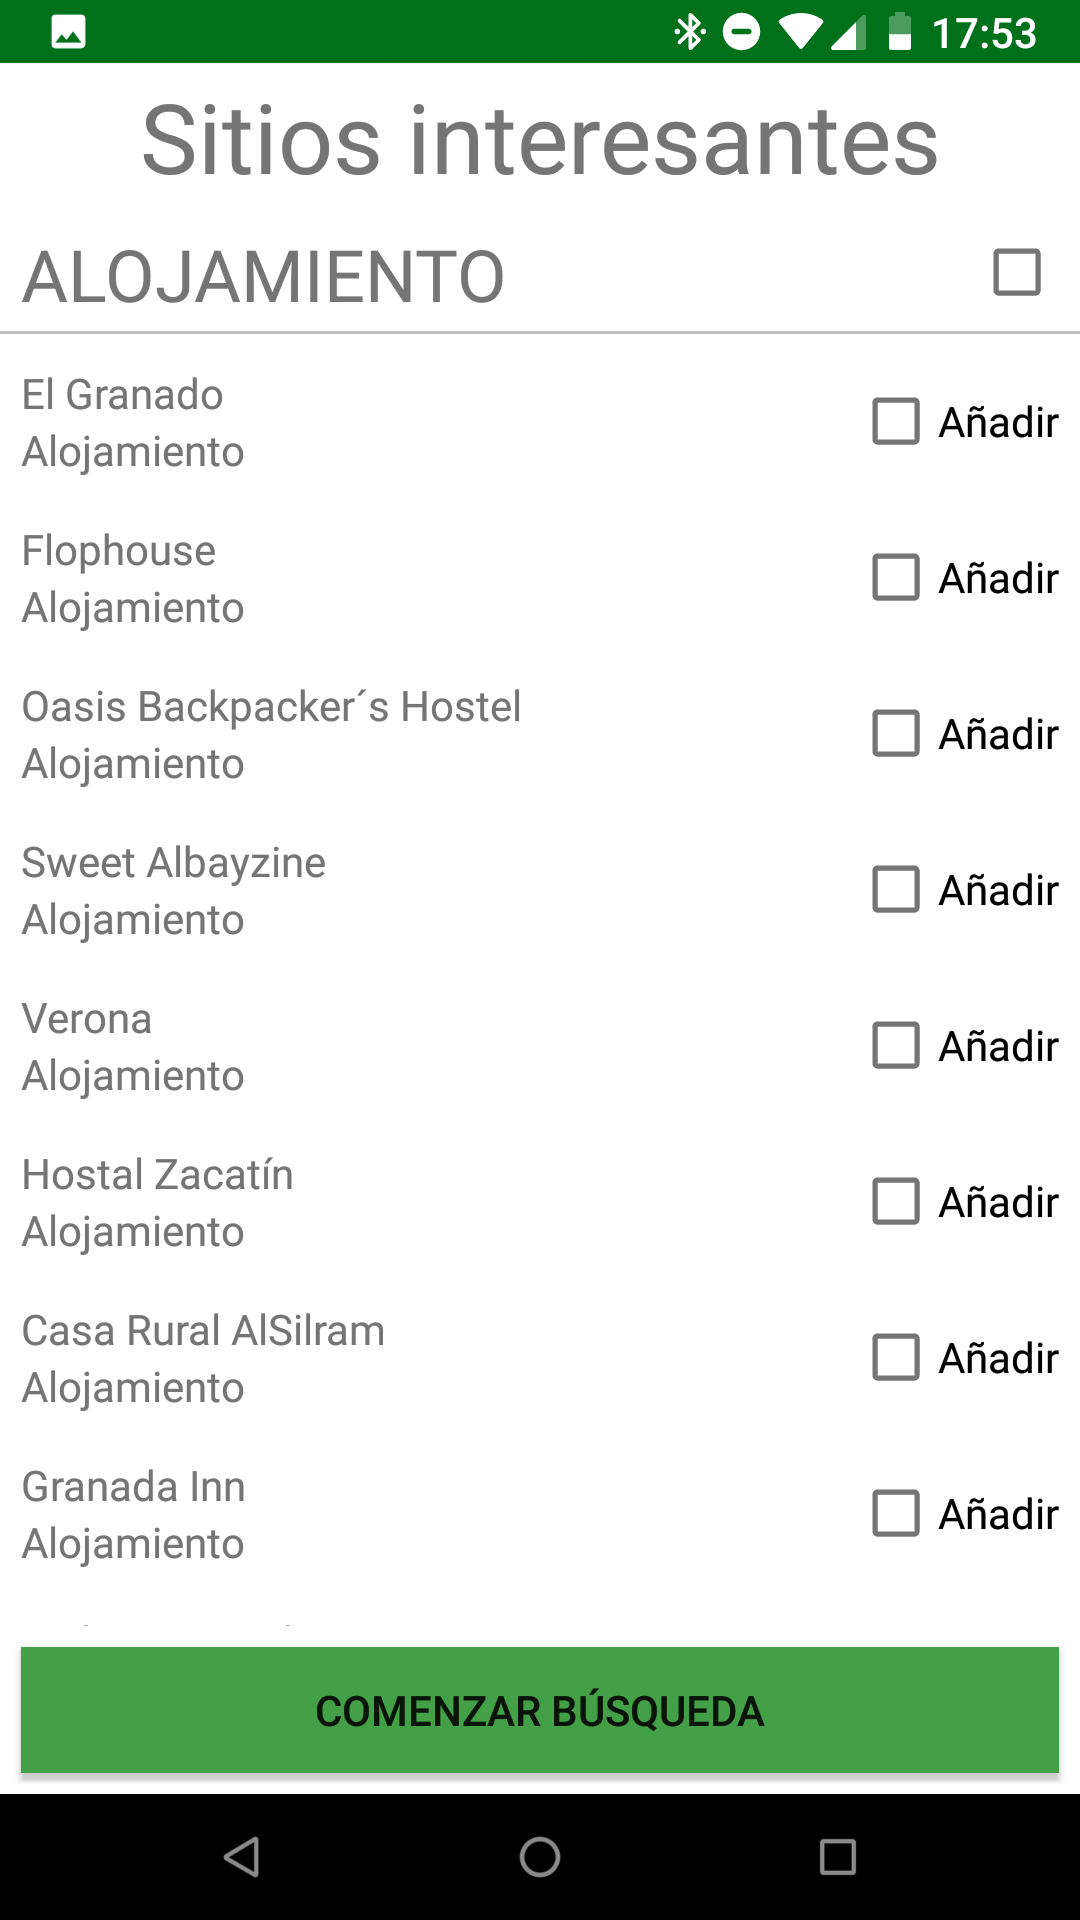
\includegraphics[width=50mm]{imagenes/main_activity_list}}
	\subfigure{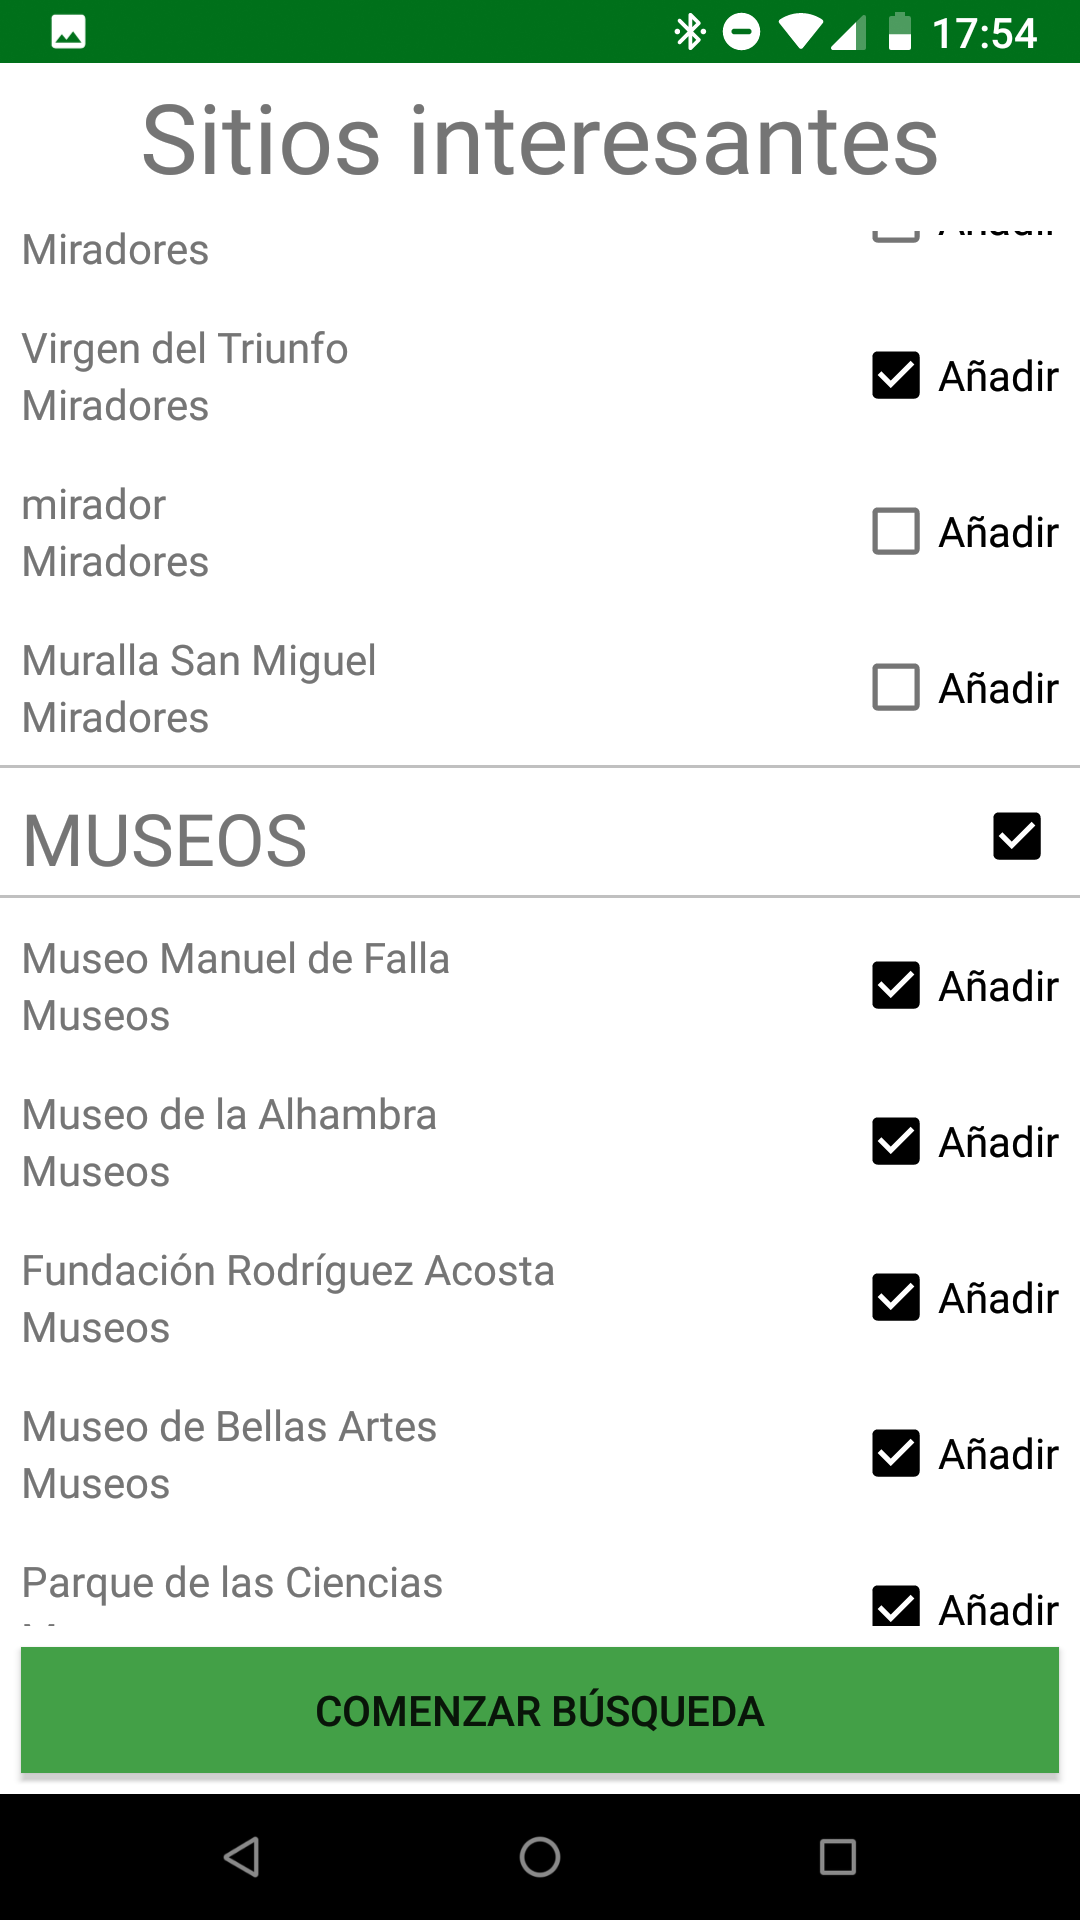
\includegraphics[width=50mm]{imagenes/main_activity_list_2}}
	\caption{Lista de alojamientos y POIs disponibles para seleccionar.}
	\label{fig:main_activity_list}
\end{figure}

\vspace{0.06in}
\begin{figure}
	\centering
	\subfigure{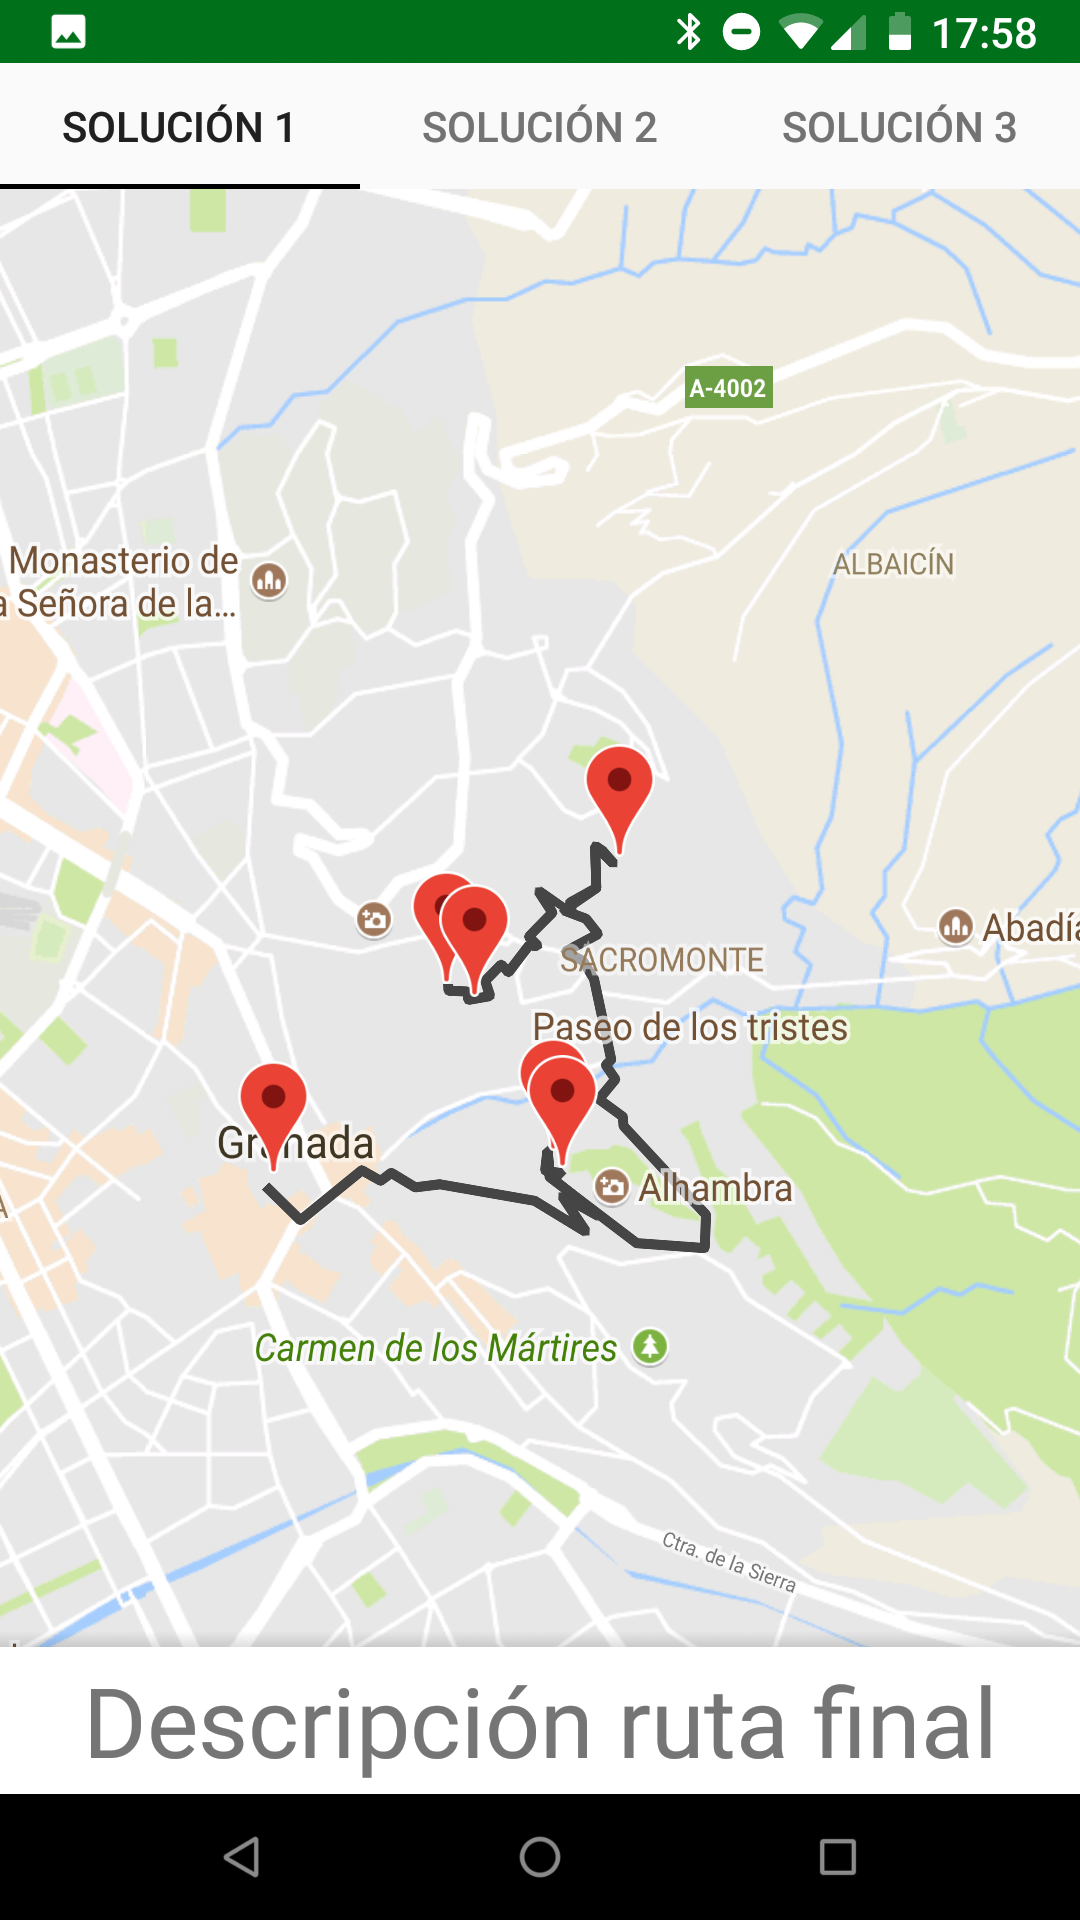
\includegraphics[width=50mm]{imagenes/solution}}
	\subfigure{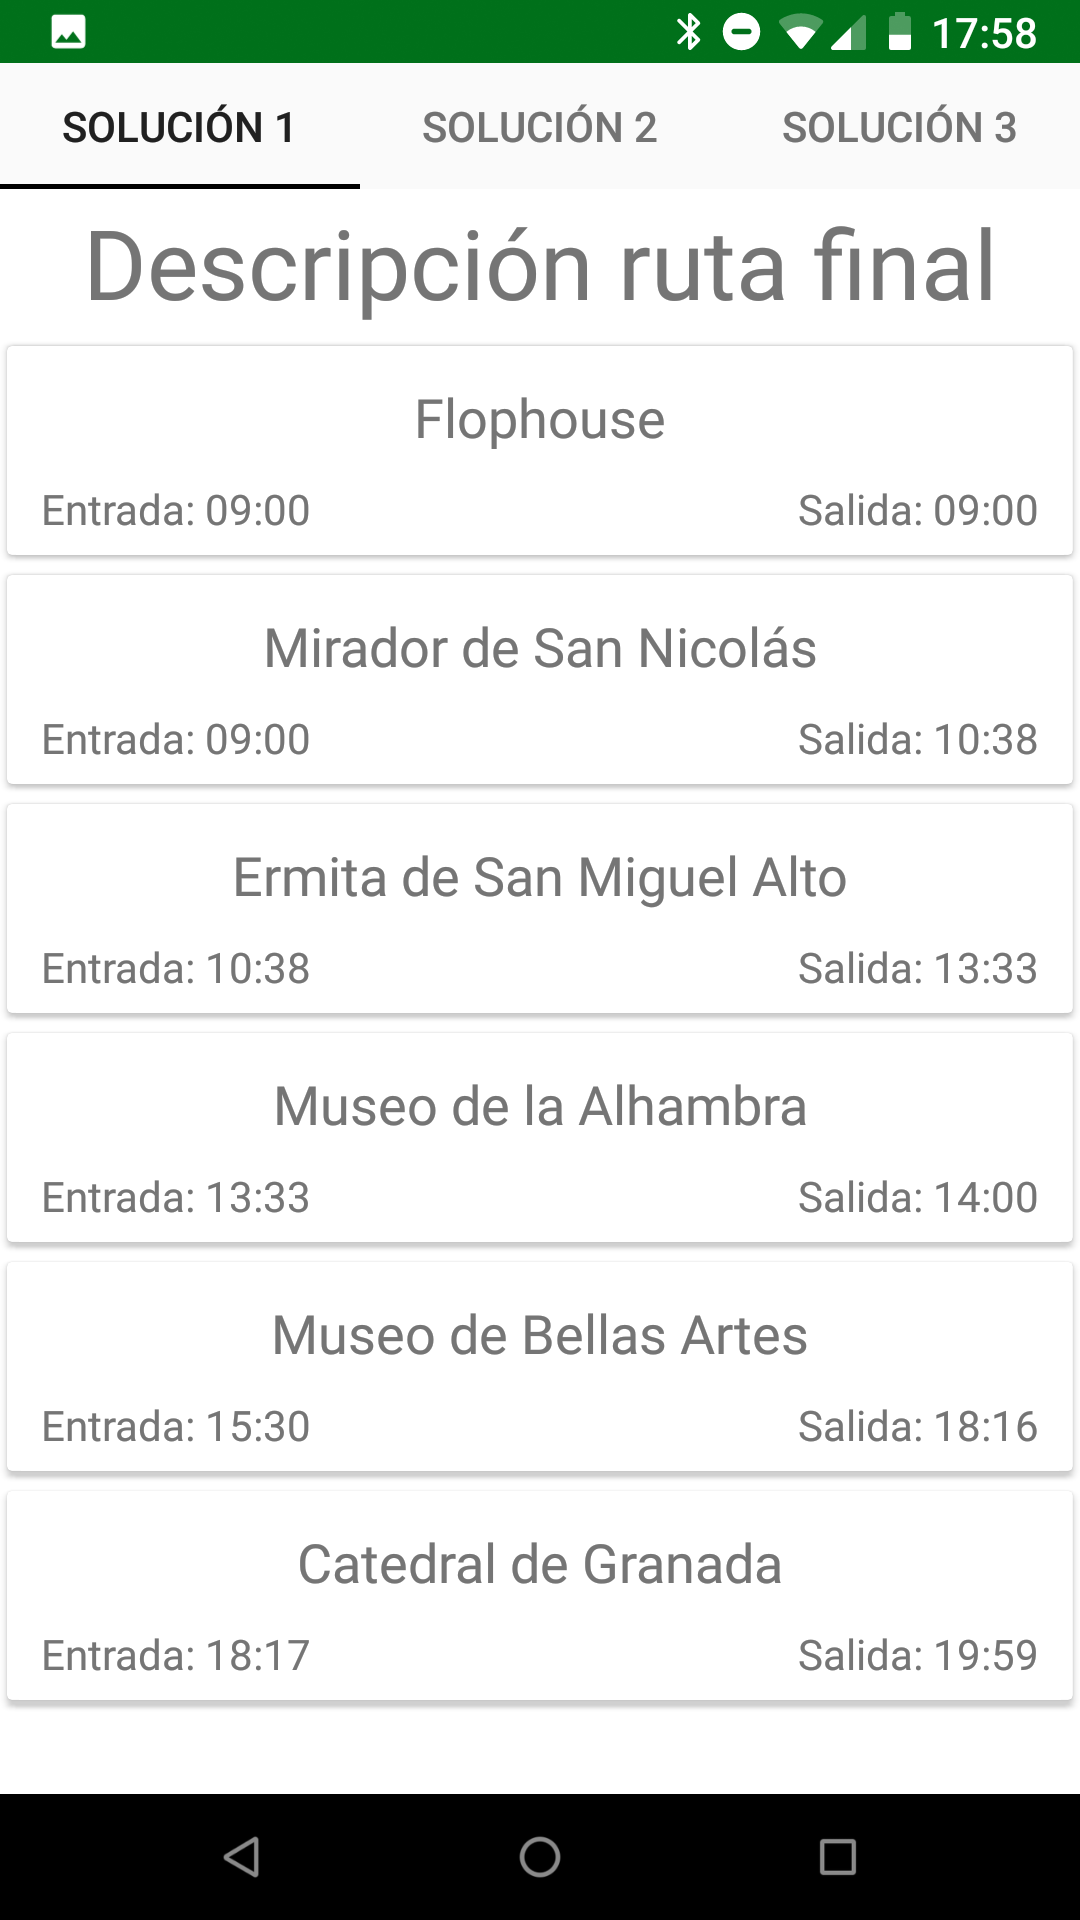
\includegraphics[width=50mm]{imagenes/list_solution}}
	\caption{Mapa mostrando solución y lista de POIs de la solución.}
	\label{fig:result_activity}
\end{figure}
